%!TEX root = ../thesis.tex
% створюємо розділ
\chapter{Генеративні моделі у задачах сегментації супутникових знімків}
\label{chap:gans}

У другому розділі ми розглянемо генеративні моделі, які можуть
бути застосовані для генерації штучних супутникових знімків.
Особлива увага буде приділена генеративно-змагальним нейронним
мережам. Також піде мова про вирішення задачі image-to-image translation
за допомогою GAN, а саме про архітектуру Pix2Pix та її вдосконалені версії.
Та нарешті буде описано механізм застосування генеративно-змагальних мереж
для аугментації навчальних вибірок, що має за мету вирішити проблеми, які
були описані у попередньому розділі.

\section{Різновиди генеративних моделей}

Для того, щоб наблизитись до розв'язку проблеми генерації
штучних зображень,
розглянемо наступну задачу:
нехай існує набір даних $(x_1, x_2, \dots) \in X$,
які мають невідомий розподіл $\pi$.
Ми намагаємось знайти його оцінку
$$p^* \in \arg \min\limits_{p} \mathcal{D}(\pi || p),$$
де $\mathcal{D}$ - деяка
міра близькості розподілів, яка задовольняє умови
\begin{equation*}
    \begin{cases}
        \mathcal{D}(\pi || p) \geq 0, & \pi \neq p \\
        \mathcal{D}(\pi || p) = 0,    & \pi = p
    \end{cases}
\end{equation*}

Наприклад дивергенція Йонсена-Шеннона:
\begin{equation} \label{eq:jsd}
    JSD(\pi || p) = \frac{1}{2} \int\limits_{\mathbb{R}}
    \left[
        \pi(x) \ln \frac{2\pi(x)}{p(x) + \pi(x)} +
        p(x) \ln \frac{2p(x)}{p(x) + \pi(x)}
        \right] dx
\end{equation}

Якщо ми зможемо знайти дану оцінку розподілу для
реальних супутникових знімків, то ми зможемо
генерувати випадкові величини з даного розподілу, які
і будуть являти собою штучні знімки. Звичайно, що
пошук по усім можливим розподілам є дуже складною задачею,
тому ми зосередимось на параметричних моделях, тобто:
$$p(x | \theta) \in \arg \min\limits_{\theta} \mathcal{D}(\pi || p_\theta),$$

Існує багато методів розв'язку подібних задач, які можна поділити
на декілька великих груп \cite{goodfellow2016nips},
що зображено на рис. \ref{fig:gen_models}.

\begin{figure}[!ht]
    \centering
    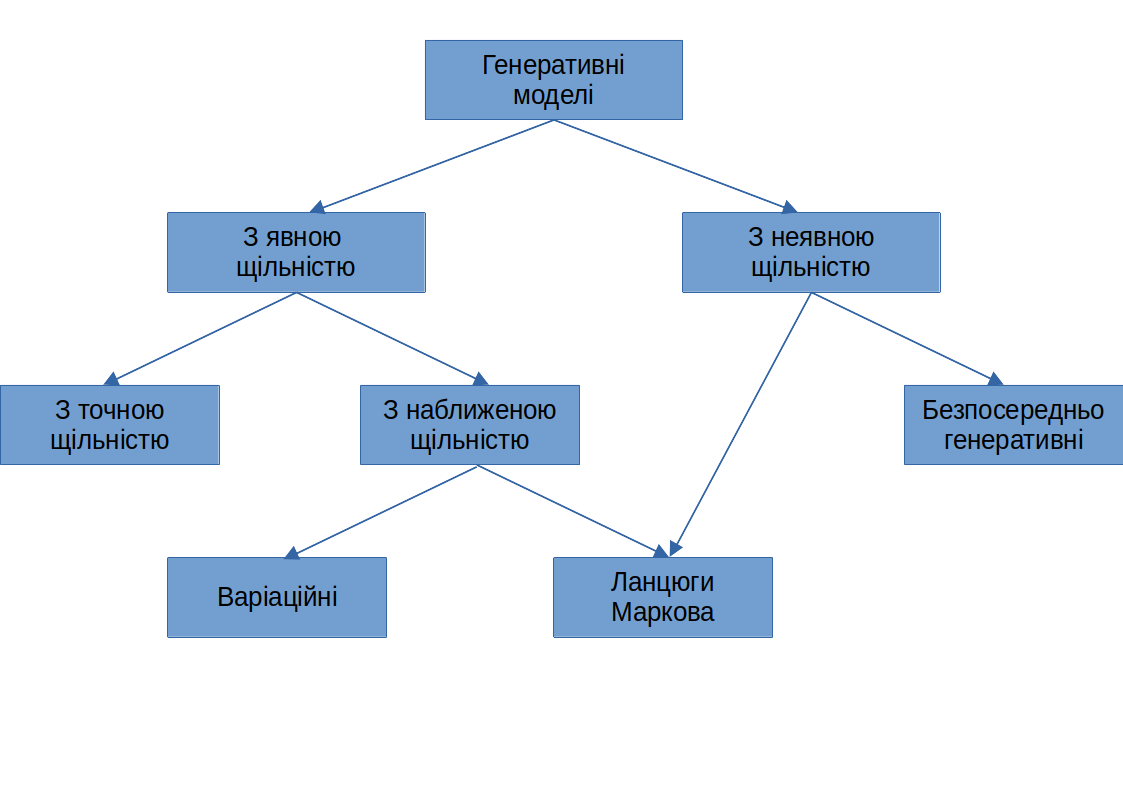
\includegraphics[width=0.9 \textwidth]{gen_models.png}
    \caption{Таксономія генеративних моделей}
    \label{fig:gen_models}
\end{figure}

Моделі з явною щільністю дозволяють обраховувати значення щільності.
Максимізація правдоподібності для даних моделей є простою,
бо являє собою просту підстановку щільності, що описує модель,
у вираз для правдоподібності. Найскладніше для даної групи
підібрати таку модель, яка зможе описувати усю складність реальних даних
і при цьому дозволить обраховувати щільність розподілу.
Тому виділяють дві стратегії:
\begin{enumerate}
    \item моделі, які гарантують можливість точного обрахунку (tractability);
    \item моделі, які ґрунтуються на обрахунку наближених значень.
\end{enumerate}

Моделі, які гарантують можливість точного обрахунку щільності, такі як
FVBN (fully visible belief networks), нормалізуючи потоки, мають перевагу у тому,
що дозволяють проводити оптимізацію безпосередньо функції
правдоподібності, проте це вимагає від них жорстких обмежень.
До того ж більшість подібних моделей виконують обрахунки послідовно,
тобто для генерації необхідно виконати декілька послідовних кроків, які
не можуть бути розпаралелині, що значно збільшує час необхідний для
генерації.

Для уникнення проблем, пов'язаних з жорсткими обмеженнями на
модель, які необхідні для точно обрахунку щільності, використовуються
моделі, які дозволяють отримувати наближені значення щільності.
Вони у свою чергу поділяються на дві групи: з детерміністичною
апроксимацією, здебільшого це автоенкодери, та зі стохастичною,
як наприклад ланцюги Маркова, машини Больцмана.

Звичайно, що і у даних підходів є суттєві недоліки.
Варіаційні автоенкодери використовують у своїй роботі
нижню границю (ELBO), яка при виборі "слабкого" апостеріорного
або ж апріорного може значно відрізнятися від справжньої
правдоподібності, що призведе до того, що розподіл генератора
та реальний розподіл будуть значно відрізнятись. На практиці
варіаційні моделі все ж здатні гарно апроксимувати правдоподібність,
проте якість згенерованих зображень є низькою. Якщо ж казати про
недоліки методів побудованих на основі ланцюгів Маркова, то
слід зазначити їх низьку швидкодію, що обумовлена як необхідністю
виконувати операції покроково, так і тим, що збіжність
дужу повільна та не має жодного методу, який би міг вказати
чи вже наявна збіжність чи потребується продовжити оптимізацію.

Концептуально іншим підходом є застосування моделей, які
не оперують щільністю або її наближеннями як такими, а
навчаються лише ґрунтуючись на тих прикладах, які надає
генератор. Тобто використовують не сам розподіл як такий, а
певні спостереження з нього. Деякі з цих моделей знову ж таки
використовують ланцюги Маркова для генерування прикладів,
здебільшого це генеративні стохастичні мережі. Але вони мають
притаманні усім ланцюгам Маркова недоліки, які були описані вище.
І на сам кінець існують моделі, які здатні безпосередньо
генерувати зображення за один крок. Найбільш відомими й поширеними з них
є генеративно-змагальні мережі, які ми розглянемо більш детально.

\section{Генеративно-змагальні мережі}

Ідея оригінального GAN  \cite{pix2pix}
полягає у тому, що ми маємо дві сутності:
генератор --- диференційовну функцію $G: Q \times \Theta_G \rightarrow X$, яка
на основі елементу з множини $Q$ (так званого латентного простору)
та параметрів $\theta_g \in \Theta_G$
генерує елемент з множин $X$; та дискримінатор
--- диференційовну функцію $D: X \times \Theta_D \rightarrow \{0, 1\}$, яка
намагається на визначити чи є елемент штучно згенерованим, чи
належить розподілу навчальних даних. Для пошуку функції
генератора та дискримінатора застосовується міні-максний функціонал якості:
\begin{equation} \label{eq:gan_criterion}
    \min\limits_{G}\max\limits_{D} \left[
        \E_{x \sim \pi} \ln D(x) +
        \E_{q \sim p_{Q}} \ln (1 - D(G(q))) \right],
\end{equation}

Тобто відбувається змагання між генератором, який прагне генерувати найбільш
схожі на реальні зображення, щоб ввести в оману дискримінатор,
який навпаки прагне якомога краще відрізняти штучно згенеровані та
реальні приклади.

Але для того, щоб знайти відповідні оптимальні значення
параметрів дискримінатора та генератора необхідний алгоритм навчання,
який з кожним кроком буде все ближче і ближче наближати розподіл
генератора до реального, аж поки дискримінатор не втратить будь-яку можливість
відрізняти реальні та штучно згенеровані зображення. Дану ідею
зображено на рис. \ref{fig:gan}.

\begin{figure}[h]
    \centering
    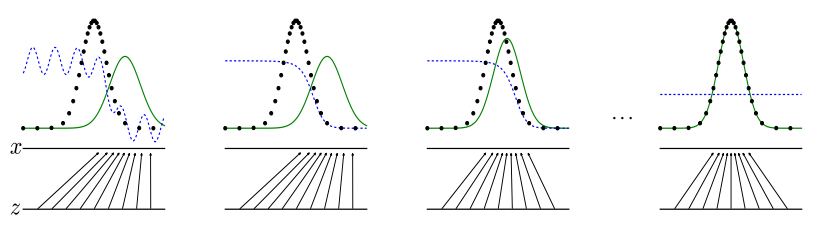
\includegraphics[width=0.75 \textwidth]{gan_distribution.png}
    \caption{Ілюстрація ідеї GAN \cite{goodfellow2014generative}.
        Зеленим позначено розподіл генератора,
        синім --- дискримінатора,
        чорними точками --- реальних даних}
    \label{fig:gan}
\end{figure}

Як це притаманно
штучним нейронним мережам, алгоритм оптимізації ґрунтується на
обрахунку і використанні градієнтів цільової функції помилки
від параметрів. Але, через те, що наша модель не є класичною
нейромережею, необхідний окремий підхід до навчання GAN.

\begin{algorithm}[Алгоритм навчання GAN]

    Параметри: $k$ - кількість ітерацій навчання дискримінатора за 1 епоху,
    $N$ - кількість епох навчання, $m$ - розмірність батчу.

    Вхідні дані: навчальна вибірка $X$ з розподілом $\pi$.

    \begin{enumerate}
        \item Доки кількість епох навчання не досягла $N$
              \begin{enumerate}
                  \item Повторювати $k$ разів
                        \begin{enumerate}[leftmargin=3.25cm]
                            \item Згенерувати $\{z_1, \dots, z_m\}$
                            \item Обрати $\{x_1, \dots, x_m\} \sim \pi(x)$
                            \item Оновити параметри дискримінатора використовуючи градієнт
                                  \begin{equation*}
                                      \nabla_{\theta_D} \left( \frac{1}{m}\sum\limits_{i=1}^m \left[
                                              \ln D(x_i) + \ln (1 - D(G(z_i))) \right] \right)
                                  \end{equation*}
                        \end{enumerate}
                  \item Згенерувати нові $\{z'_1, \dots, z'_m\}$\;
                  \item Оновити параметри генератора використовуючи градієнт
                        \begin{equation*}
                            \nabla_{\theta_G} \left( \frac{1}{m}\sum\limits_{i=1}^m
                            \ln (1 - D(G(z'_i))) \right)
                        \end{equation*}
              \end{enumerate}
    \end{enumerate}
\end{algorithm}

У якості оптимізатора, який використовує вже обраховані градієнти
можна застосовувати довільний алгоритм, у більшості випадків це або
звичайний градієнтний спуск,
або більш досконалі методи, як наприклад
Adam \cite{kingma2014adam}.

Окремим питанням, яке заслуговує на увагу, є питання про те,
а чи дійсно у результаті розв'язку цієї задачі ми отримаємо
генератор, розподіл якого дорівнює розподілу реальних даних.
Для того, щоб переконатися у цьому доведемо дві важливі теореми.

\begin{theorem}[Гудфелоу \cite{goodfellow2014generative}]
    Для фіксованого генератора $G$ з розподілом $p_G(x)$
    оптимальним дискримінатором $D^*(x)$ є:
    \begin{equation*}
        D^{*}(x) = \frac{\pi(x)}{\pi(x) + p_G(x)}.
    \end{equation*}
\end{theorem}
\begin{proof}
    Запишемо цільову функцію:
    \begin{equation*}
        \min\limits_{G}\max\limits_{D} \left[
            \E_{x \sim \pi} \ln D(x) +
            \E_{q \sim p_{Q}} \ln (1 - D(G(q))) \right]
    \end{equation*}
    Генератор, за припущенням є фіксованим, тож ми можемо перейти
    від математичного сподівання по латентному просторі до математичного сподівання
    розподілу генератора $p_G(x)$.
    \begin{equation*}
        \min\limits_{G}\max\limits_{D} \left[
            \E_{x \sim \pi} \ln D(x) +
            \E_{x \sim G(x)} \ln (1 - D(x)) \right]
    \end{equation*}
    Наступним кроком розпишемо математичні сподівання та
    властивостями визначених інтегралів:
    \begin{equation*}
        \min\limits_{G} \int\limits_X \max\limits_{D}
        \left( \pi(x) \ln D(x) +
        p_G(x) \ln (1 - D(x)) \right) dx
    \end{equation*}
    Розглянемо умову екстремум для виразу під
    знаком максимуму і отримаємо:
    \begin{gather*}
        \frac{\partial}{\partial D(x)}
        \left( \pi(x) \ln D(x) +
        p_G(x) \ln (1 - D(x)) \right) = \\
        = \frac{\pi(x)}{D(x)} - \frac{p_G(x)}{1 - D(x)} = 0
    \end{gather*}
    І виразивши $D(x)$ остаточно отримаємо:
    \begin{equation*}
        D^{*}(x) = \frac{\pi(x)}{\pi(x) + p_G(x)}
    \end{equation*}
\end{proof}

\begin{theorem}[Гудфелоу \cite{goodfellow2014generative}]
    Глобальний мінімум критерію \eqref{eq:gan_criterion} досягається
    тобі і тільки тоді, коли розподіли генератора $p_G$ та реальних даних
    однакові. При цьому значення критерію дорівнює $-\ln 4$.
\end{theorem}
\begin{proof}
    Підставимо оптимальний дискримінатор у критерій~\eqref{eq:gan_criterion}.
    \begin{equation*}
        \min\limits_{G} \left[
            \E_{x \sim \pi} \ln \frac{\pi(x)}{\pi(x) + p_G(x)} +
            \E_{q \sim p_G} \ln \frac{\pi_G(x)}{\pi(x) + p_G(x)}
            \right]
    \end{equation*}
    Тепер помножимо і поділимо кожен дріб на 2 та використаємо властивість
    логарифмів та математичного сподівання від константи.
    \begin{equation*}
        \min\limits_{G} \left[
            \E_{x \sim \pi} \ln \frac{2 \pi(x)}{\pi(x) + p_G(x)} +
            \E_{q \sim p_G} \ln \frac{2 \pi_G(x)}{\pi(x) + p_G(x)}
            \right] - \ln 4
    \end{equation*}
    Вираз у дужках є нічим іншим як дивергенцією Йонсена-Шеннона \eqref{eq:jsd}.
    Вона приймає мінімальне значення $0$ тоді і тільки тоді, коли
    розподіли дорівнюють один одному. І, відповідно, значення критерію
    у випадку рівності $0$ мінімуму буде дорівнювати $-\ln 4$.
\end{proof}

Проте наявний алгоритм навчання майже завжди не використовується
на практиці, що пов'язано з тим, що градієнти параметрів генератора
згасають \cite{arjovsky2017towards, goodfellow2014generative}.
Це є наслідком самої будови функції помилки, тому її заміняють
на наступний аналог:

\begin{equation} \label{eq:gan_generator_loss}
    - \ln D(G(z))
\end{equation}

Притаманні процесу навчання генеративно-змагальних мереж і інші проблеми,
як наприклад нестабільність навчання, яка полягає у тому, що
у деяких випадках алгоритм не може знайти оптимальні
дискримінатор та генератор. Деякі причини цього детально
описані у роботі \cite{arjovsky2017towards}, серед них нестабільність
градієнтів функції помилки у вигляді \eqref{eq:gan_generator_loss}.
Іншою можливою причиною може бути те, що як зображено на рис. \ref{fig:gan},
з кожною ітерацією генератор покращується, що робить зворотній
зв'язок від дискримінатора все менш правильним, і на сам кінець зовсім випадковим.
Тобто генератор починає вчитися на небажаному зворотному зв'язку від дискримінатора.

Одним зі шляхів подолання даних проблем є додавання шуму до
входу дискримінатора, застосування спектральних нормалізацій \cite{miyato2018spectral} або
ж регуляризацій \cite{roth2017stabilizing}.

Іншою істотною проблемою є так званий mode collapse.
Вона полягає у тому, що вихідні зображення дуже мало
відрізняються один від одного та модель не в змозі генерувати
різноманітні приклади. Це відбувається через те, що генератор
завжди намагається ввести в оману дискримінатор, і для цього
генерує зображення, які з найбільшою ймовірністю будуть розпізнанні
дискримінатором як справжні. Але якщо виявилось так, що
дискримінатор потрапив у локальний максимум, з якого не може вибратись,
то генератор надмірно пристосовується саме до цього дискримінатора, через
що і генерує невелике розмаїття зображень.

Зміна дискримінатора та критерію оптимізації спроможні подолати
дану проблему. Одним з таких підходів є Wasserstein GAN \cite{arjovsky2017wasserstein}.
Який змінює дискримінатор, який приймає обмежені значення на критика,
виходи якого можуть бути довільні. До того ж сама функція помилки
була змінена на таку, що відображає відстань між розподілами.
Серед усього іншого, даний підхід спроможний допомогти і
у випадку нестабільного навчання.

Попри усі згадані недоліки, якість зображень та швидкодія генерації
штучних прикладів для генеративно-змагальних мереж є
високою, що і робить GAN визнаним спільнотою лідером у задачах
генерації штучних зображень.

Підсумовуючи, генеративно-змагальні мережі мають наступні
переваги над іншими моделями:
\begin{enumerate}
    \item Можливість паралельної генерації,
          що забезпечує швидкість роботи навченої моделі.
    \item На генератора накладається мало обмежень, що дає можливість
          вибору широко класу архітектур.
          Це є перевагою порівняно з машинами Больцмана,
          які допускають лише певні класи  ймовірнісних розподілів,
          а також щодо потоків, що нормалізують, які вимагають, щоб генератор
          мав зворотнє відображення, а розмірність латентного простіру
          дорівнювала розмірності даних.
    \item Не використовуються ланцюги Маркова з усіма їх
          недоліками, як у машинах Больцмана та генеративних стохастичних мережах.
    \item Генеративна мережа, оптимізація якої була збіжною, точно наближає
          розподіл реальних даних, а не використовує нижні чи верхні
          оцінки, як це у випадку з автоенкодерами.
    \item Якість зображень, які генеруються за допомогою GAN,
          здебільшого вища за інші моделі.
\end{enumerate}

Саме ці моменти і обумовлюють вибір саме генеративно-змагальних
мереж для генерації штучних супутникових знімків, і, як наслідок,
аугментації навчальних вибірок.

\section{GAN у задачах image-to-image translation}

\begin{figure}[ht]
    \centering
    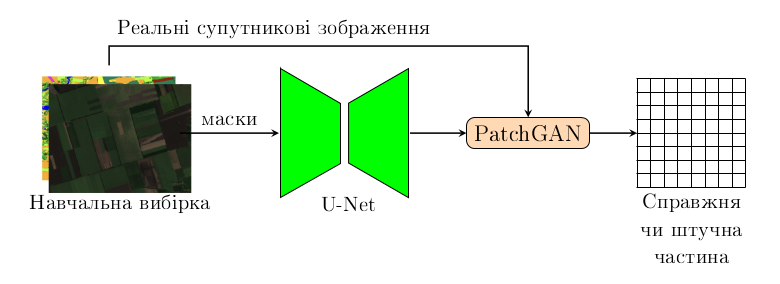
\includegraphics[scale=0.5]{pix2pix.png}
    \caption{Архітектура Pix2Pix у застосуванні до супутникових знімків}
    \label{fig:pix2pix}
\end{figure}

\section{Перспективи застосування GAN для генерації штучних супутникових знімків}

\begin{figure}[ht]
    \centering
    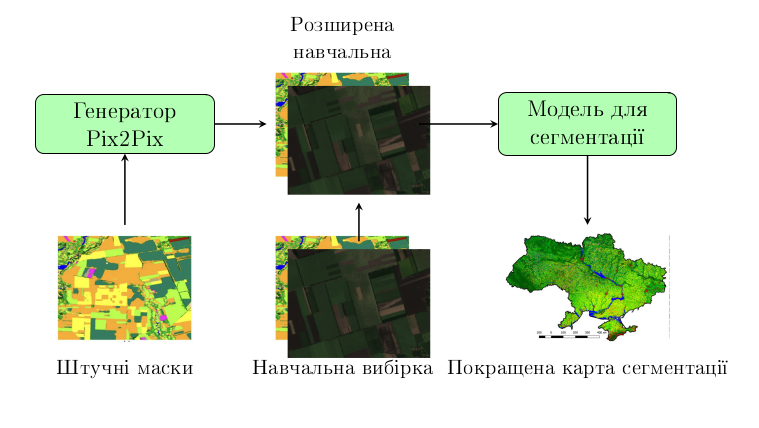
\includegraphics[scale=0.5]{pipline.png}
    \caption{Процес аугментації наборів даних супутникових знімків за допомогою Pix2Pix}
    \label{fig:pipline}
\end{figure}



\chapconclude{\ref{chap:gans}}

Був запропонований процес аугментації навчальних вибірок супутникових
знімків, який полягає у тому, що ми, за описаним алгоритмом, спершу
генеруємо маски, які будуть коригувати незбалансованість класів,
а після цього, ґрунтуючись на даних масках генерувати штучні
супутникові знімки за допомогою
архітектури Pix2Pix та її варіацій.